\section{Ocean Dissipation in Titan \label{sec:results_Titan}}

The following results are split into three main sections. Firstly, we compare dissipation between Rayleigh drag (section \ref{sec:ray_titan}) and bottom drag (section \ref{subsec:botTitan}) for Titan. Section \ref{subsec:scalTitan} then compares the bottom drag results to scaling laws from \citet{chen2013tidal}. We repeat these results for Enceladus in section \ref{sec:results_Enceladus}.

\subsection{Rayleigh Drag}\label{sec:ray_titan}

Dissipated surface heat flux averaged over the tidal period was calculated over $h_0$ and $\alpha$ space for each main tidal component, as shown in Figure \ref{fig:linTitan}. The eccentricity tide (Figure \ref{fig:lincEccTitan}) shows three resonant ocean thicknesses, $h_0 \sim$ \SIlist{2;3;22}{\metre}. These horizontal resonances are the result of excited gravity waves, with the deepest of these having a maximum dissipated surface heat flux of $\sim 10\, \si{\watt\per\square\metre}$ which occurs between $\alpha =$ \SIrange{e-8}{e-7}{\per\second}. Notably, the maximum dissipated energy does not occur for the most drag dominated oceans where $\alpha \sim \num{e-5} \, \si{\per\second}$. 

\begin{figure*}[!t]
    \centering
    \begin{subfigure}[t]{0.95\linewidth} % contains the two plots in a single figure
        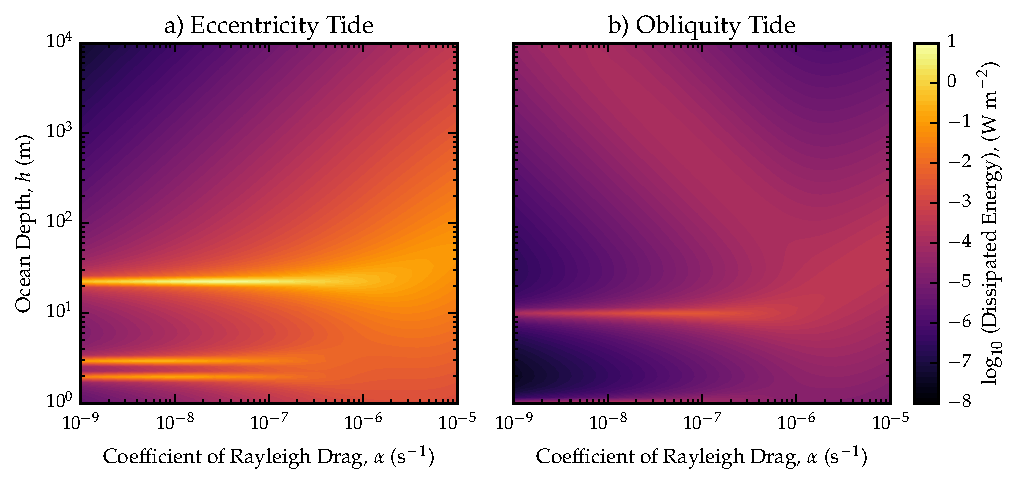
\includegraphics[width=\linewidth]{Figures/titan_linear}
        \phantomcaption
        \label{fig:lincEccTitan}
    \end{subfigure}
    \begin{subfigure}[t]{0\linewidth} % the hidden unwanted image
         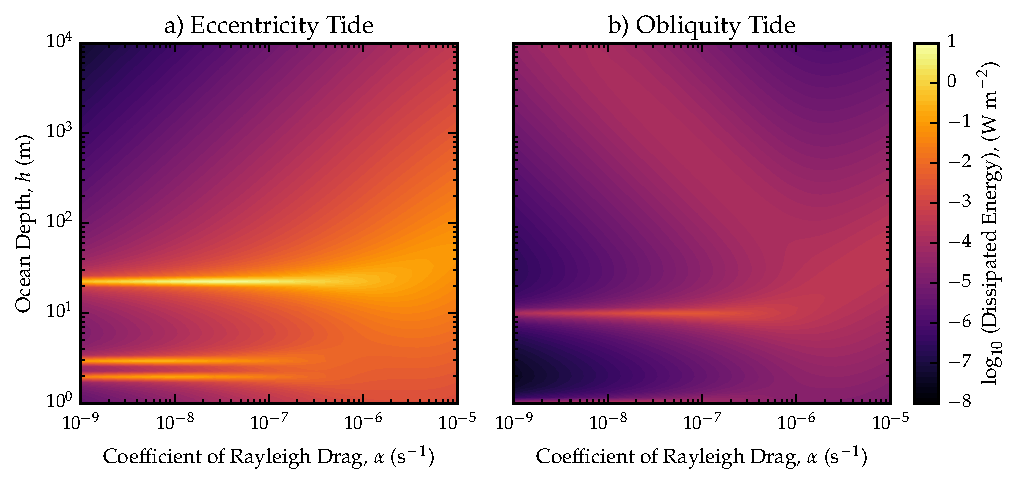
\includegraphics[width=\linewidth]{Figures/titan_linear}
         \phantomcaption
         \label{fig:linObliqTitan}   
    \end{subfigure}
    \vspace{-0.5cm}
\caption{Global ocean surface dissipation solutions for Titan under the eccentricity (left) and obliquity (right) tides. The logarithm of dissipated energy flux is shown as a function of ocean thickness, $h_0$, and Rayleigh drag coefficient, $\alpha$. All simulations were performed with \SIrange{2}{3}{\degree} resolution.}
\label{fig:linTitan}
\end{figure*}

Figure \ref{fig:linObliqTitan} illustrates the dissipated surface heat flux for the obliquity tide on Titan. Two resonant ocean thicknesses are found for this tidal component, $h_0 \sim$ \SIlist{1;10}{\metre}. The latter resonance is the most dissipative with an average surface heat flux of $\sim \num{4e-3}\, \si{\watt\per\square\metre}$. There is also an excited Rossby-wave resonance orientated diagonally across $h_0 \sim$ \SIrange{10}{e4}{\metre} and \hbox{$\alpha \sim$ \SIrange{e-6}{e-9}{\per\second}}. The maximum average surface heat flux occurring along the length of this resonance is $\sim \SI{e-4}{\watt\per\square\metre}$. 

Numerical error over this parameter space was also computed using the semi-analytical solutions from \citet{matsuyama2014tidal}. The eccentricity tide is accurate to within \SI{1}{\percent} over much of the parameter space, with resonances being the least accurate (in terms of absolute value). Resonances that occur in the thickest oceans differ from the analytical solution by \SIrange{1}{20}{\percent}. We ignore discrepancies in thin oceans ($h_0 \leq 10 \, \si{\metre}$) as bathymetry of the ocean floor for any icy satellite will likely be comparable to or exceed the ocean thickness, directly violating the assumptions made in the LTEs. It should also be noted that resonances found below $h_0 = 10 \, \si{\metre}$ typical have displacements greater than the thickness of the ocean. \textbf{While such situations clearly have no physical meaning, they are nonetheless mathematically possible. We therefore cannot consider the results in this part of the parameter space. It should be noted that for best comparison of the numerical model to the \citet{matsuyama2014tidal} solutions, it is still useful to solve this part of the parameter space, even if the results are unphysical. The small amplitude assumption, discussed in section \ref{subsec:LTE}, is almost certainly a factor that allows the development of such large tidal displacements in the numerical and semi-analytical solutions. This is because non-linearities in the model are unable to play a more significant role in the solution. In this work, it is important to include this assumption for best verification of the numerical results with the semi-analytical solutions. Future versions of ODIS shall proceed without the small amplitude assumption.}

\subsection{Bottom Drag \label{subsec:botTitan}}

Dissipation across $h_0$ and $c_D$ space (bottom drag) is shown in Figure \ref{fig:botTitan}. Tidal dissipation due to the eccentricity tide is shown in the left hand panel. Comparing this to Rayleigh drag dissipation in Figure \ref{fig:lincEccTitan} highlights some of the major differences and similarities between the two drag regimes. The resonant peaks at \SIlist{2;3;22}{\metre} from the Rayleigh drag case are all present, although they have smaller magnitudes. The resonance broadens towards larger $c_D$, and remains very diffuse over much of the parameter space. This differs from the Rayleigh drag case where the resonances are very narrow and pronounced over most of $\alpha$ space (Figure \ref{fig:lincEccTitan}). Additionally, away from the resonances and in the thickest oceans, dissipated energy drops by \numrange{10}{12} orders of magnitude when applying bottom drag, which is far smaller than the lowest dissipation found in the Rayleigh drag case.  

\begin{figure*}[!b]
    \centering
    \begin{subfigure}[t]{0.95\linewidth} % contains the two plots in a single figure
        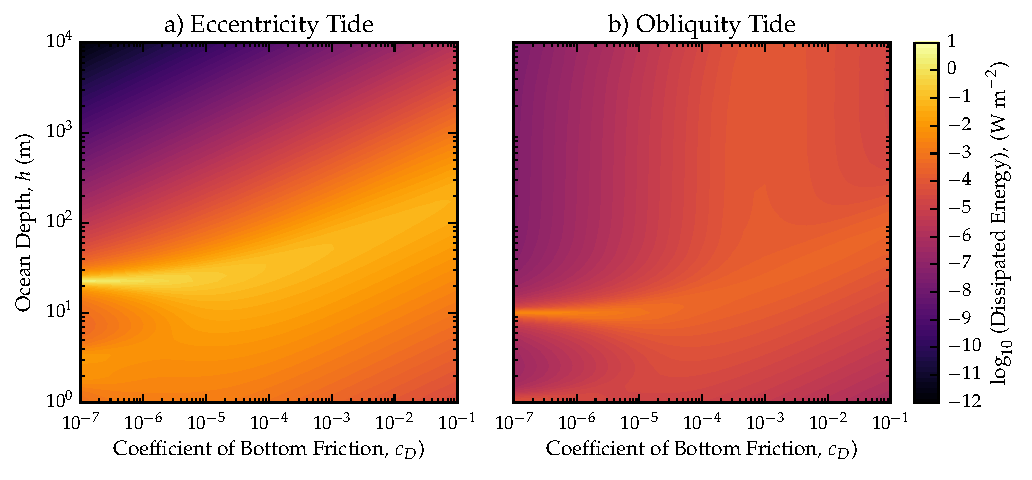
\includegraphics[width=\linewidth]{Figures/titan_bottom}
        \phantomcaption
        \label{fig:botEccTitan}
    \end{subfigure}
    \begin{subfigure}[t]{0\linewidth} % the hidden unwanted image
         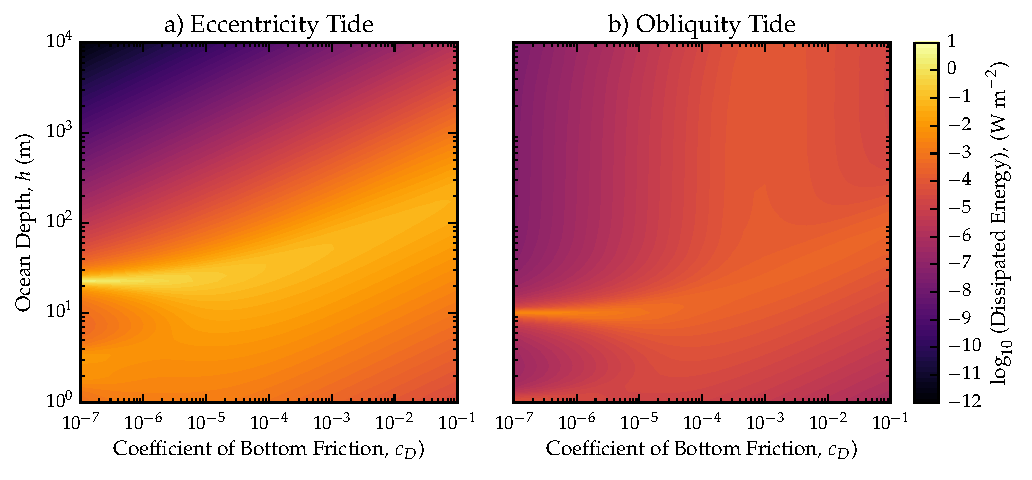
\includegraphics[width=\linewidth]{Figures/titan_bottom}
         \phantomcaption
         \label{fig:botObliqTitan}   
    \end{subfigure}
    \vspace{-0.5cm}
\caption{Global ocean surface dissipation solutions for Titan under the eccentricity (left) and obliquity (right) tides. The logarithm of dissipated energy is shown as function of ocean thickness, $h_0$, and coefficient of bottom drag, $c_D$. All simulations were performed with \SIrange{1}{3}{\degree} resolution. \label{fig:botTitan}}
\end{figure*}


Ocean dissipation under the obliquity tide using bottom drag also has several important differences and similarities to the Rayleigh case. Comparing figures \ref{fig:botObliqTitan} and \ref{fig:linObliqTitan}, it is again evident that the horizontal gravity-wave resonances at \SIlist{1;10}{\metre} are present in both solutions. The most striking difference is the orientation of the broad Rossby-wave resonance that extends into the thickest oceans. In the Rayleigh case, this resonance moves diagonally across a large region of the parameter space, whereas it is vertically oriented and limited to a small range of $c_D$ for the bottom drag case, such that the resonance becomes independent of ocean thickness. The resonance also happens to occur across the empirically derived Earth value for $c_D = 0.002$ \citep[e.g.,][]{sohl1995tidal,egbert2001estimates}. 

\subsection{Comparison with Scaling Laws \label{subsec:scalTitan}}

\begin{figure*}[!t]
    \centering
    \begin{subfigure}[t]{0.95\linewidth} % contains the two plots in a single figure
        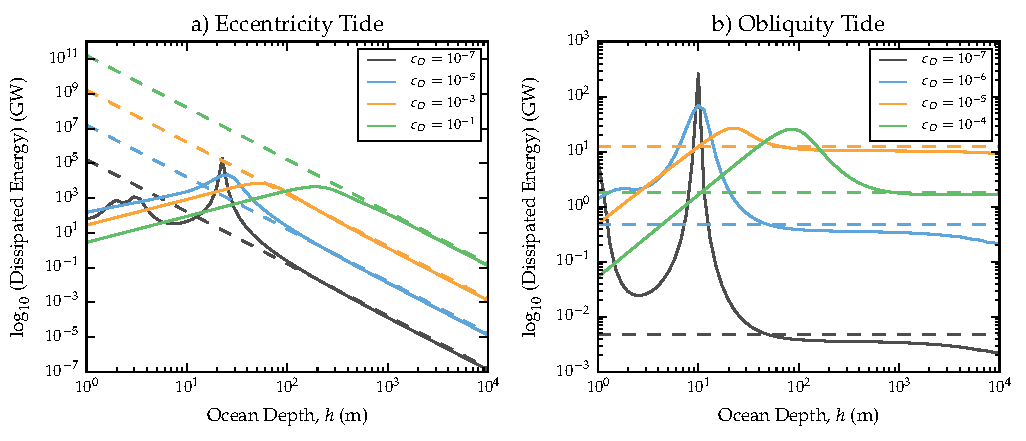
\includegraphics[width=\linewidth]{Figures/titan_scaling}
        \phantomcaption
        \label{fig:scalEccTitan}
    \end{subfigure}
    \begin{subfigure}[t]{0\linewidth} % the hidden unwanted image
         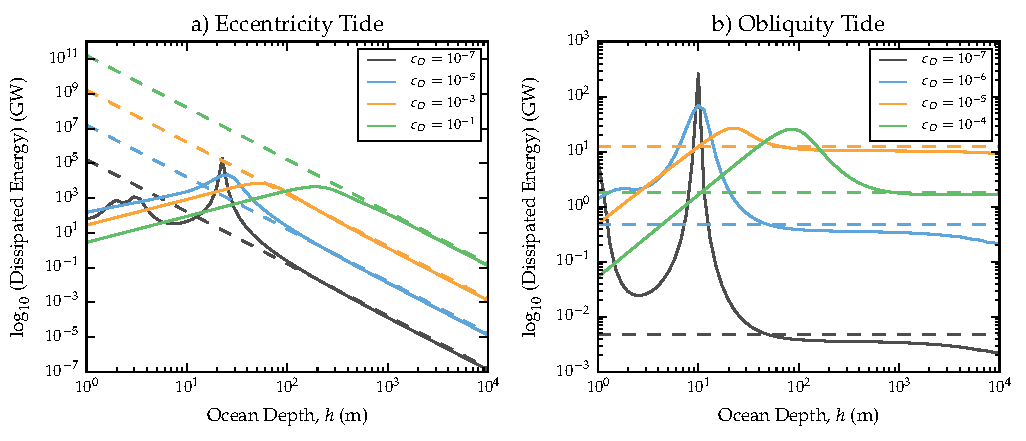
\includegraphics[width=\linewidth]{Figures/titan_scaling}
         \phantomcaption
         \label{fig:scalObliqTitan} 
    \end{subfigure}
    \vspace{-0.5cm}
\caption{Comparison of the ODIS numerical results (solid lines) and those calculated using the scaling laws (dashed lines) derived in \citet{chen2013tidal}, for Titan under the eccentricity (left) and obliquity (right) tides. The colours represent different values of bottom drag coefficient.\label{fig:scalTitan}}
\end{figure*}

While there are no fully analytical solutions to the LTEs when including bottom drag, there are a set of scaling laws for estimating dissipation that neglect gravity-wave resonant features, developed by \citet{chen2013tidal}. We compare cross sections from the results in Figure \ref{fig:botTitan} with these scaling laws, shown in Figure \ref{fig:scalTitan}.

Away from resonances and in thick oceans, there is excellent agreement between the numerical results and the scaling laws. This is particularly true of the eccentricity tide. Larger discrepancies are found for the obliquity tide (Figure \ref{fig:scalObliqTitan}) for thick oceans, but this is a result of numerical discretisation error. The vertically orientated resonant feature in Figure \ref{fig:botObliqTitan} is also produced in the scaling laws, as shown in Figure \ref{fig:scalObliqTitan}. None of the gravity-wave resonances are captured by the scaling laws. 

\subsection{Implications for Titan}

Titan likely has an ocean that is on the order of \SI{100}{\kilo\metre} thick \citep{sohl2014structural,baland2014titan}. All of the eccentricity tide resonances occur in oceans much thinner than this, suggesting that - despite the substantial free eccentricity - there is little dissipation from this tidal component in heating Titan's ocean.

Rossby-wave resonances from the obliquity tide appear as the diagonal and vertical features in figures \ref{fig:linObliqTitan} and \ref{fig:botObliqTitan}, respectively. The linear drag regime sees this resonance move into very small Rayleigh drag coefficients ($\alpha \lesssim$ \SI{e-9}{\per\second}) for oceans thicker than about \SI{10}{\kilo\metre}. However, for bottom drag, the Rossby-wave resonance is mainly independent of ocean thickness above $h_0 \gtrsim$ \SI{1}{\kilo\metre}. If Titan's ocean has a bottom drag coefficient of $c_D =$ \numrange{e-2}{e-4} then this Rossby-wave resonance would result in a total power output of \SIrange{5}{12}{\giga\watt}. The resonance therefore presents a mechanism for dissipating significant thermal energy in Titan's interior, regardless of the ocean thickness. To gain an insight into the significance of such an effect, we consider Titan's changing semimajor axis.

For a bound orbit the total energy is given as $-GMm/2a$ \citep{murray1999solar}. Differentiating this expression with respect to time gives a relationship between the dissipated energy and changing semimajor axis,
\begin{equation}
\left( \dfrac{da}{dt} \right)_t = \dfrac{2a^2}{GM m}\dfrac{dE}{dt}.
\label{eq:adot_t}
\end{equation}

where $M$ and $m$ represent the mass of Saturn and Titan, respectively. The universal gravitational constant is $G$, and dissipated energy is $dE/dt$. Note that as $dE/dt < 0$, the semimajor axis decays with time. In contrast, the semimajor axis of most bodies tends to increase over time due to tides raised by the satellite on its primary. We therefore also include the rate of change of semimajor axis due to tides raised on Saturn \citep{kaula1964tidal,goldreich1966q}:
\begin{equation}
\left( \dfrac{da}{dt} \right)_s = 3 \dfrac{k_{2s}}{Q_s}\left(\dfrac{G}{M}\right)^{\sfrac{1}{2}} \dfrac{m R_s^5}{a^{\sfrac{11}{2}}}   
\label{eq:adot_s}
\end{equation}

where the subscript $s$ denotes quantities for Saturn; the degree-2 Love number $k_{2s}$, tidal quality factor $Q_s$, and radius, $R_s$. Estimates for $k_{2s}/Q_s$ vary between approximately \numrange{e-4}{e-5} \citep{peale1980tidal,lainey2012strong}. The total time derivative of semimajor axis is then given by summing equations \ref{eq:adot_t} and \ref{eq:adot_s},
\begin{equation}
\dfrac{da}{dt} = \left( \dfrac{da}{dt} \right)_s + \left( \dfrac{da}{dt} \right)_t \, .\label{eq:adot_total}
\end{equation}

\begin{figure*}[!b]
    \centering
    \begin{subfigure}[t]{0.95\linewidth} % contains the two plots in a single figure
        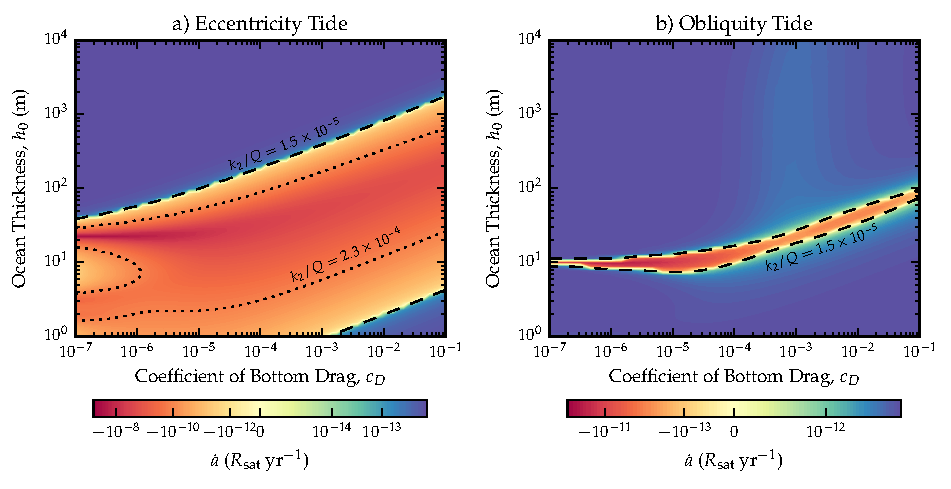
\includegraphics[width=\linewidth]{Figures/titan_adot}
        \phantomcaption
        \label{fig:a_evo_ecc}
    \end{subfigure}
    \begin{subfigure}[t]{0\linewidth} % the hidden unwanted image
         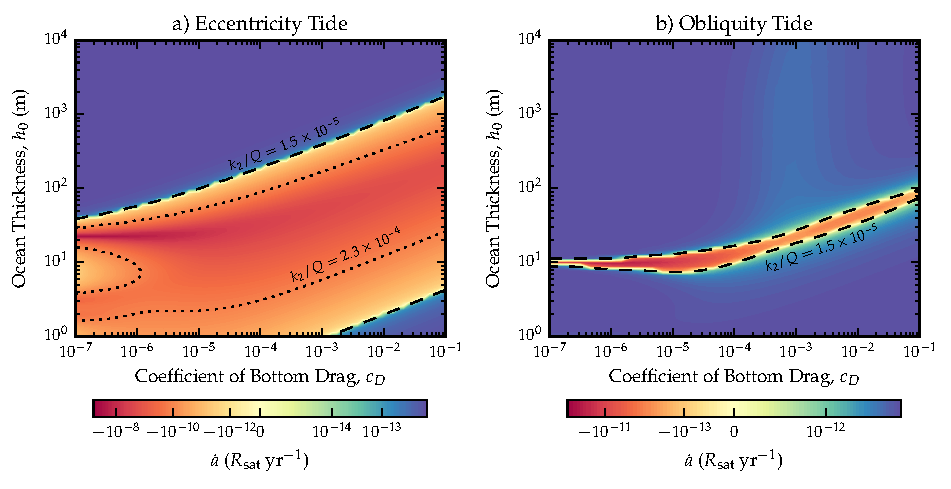
\includegraphics[width=\linewidth]{Figures/titan_adot}
         \phantomcaption
         \label{fig:a_evo_obliq} 
    \end{subfigure}
    \vspace{-0.5cm}
\caption{Rate of change of semimajor axis for Titan due to tidal dissipation in both Titan's ocean and Saturn, for each tidal component. The colour scale represents $da/dt$ assuming $k_{2s}/Q_s = \num{1.5e-5}$, where the dashed contour represents the transition from inward to outward tidal migration. The same transition is represented by the dotted contour when assuming $k_{2s}/Q_s = \num[separate-uncertainty = true]{2.3(07)e-4}$.\label{fig:a_evo}}
\end{figure*}

A plot of the total $da/dt$ from equation \ref{eq:adot_total} as a function of ocean thickness and bottom drag coefficient is shown in Figure \ref{fig:a_evo}. The colour contours are calculated using $k_{2s}/Q_s = \num{1.5e-5}$, which is approaching the upper limit of estimated $Q_s$ values \citep{peale1980tidal,meyer2007tidal}. The dotted and dashed black contours represent $da/dt=0$ \si{\Rsat\per\year} using $k_{2s}/Q_s = \num[separate-uncertainty = true]{2.3(07)e-4}$ \citep{lainey2012strong} and $k_{2s}/Q_s = \num{1.5e-5}$, respectively. The \citet{lainey2012strong} value is the most recent $k_{2s}/Q_s$ estimate for Saturn. The regions enclosed by the black contour lines represent inward migration of Titan, where $da/dt < 0$. Outside of this, the semimajor axis increases with time. 

Dissipation due to the eccentricity tide can be significant enough to reverse the outward migration of Titan when assuming either of the two $k_{2s}/Q_s$ values we have explored (Figure \ref{fig:a_evo_ecc}). The region in the $h_0$ - $c_D$ parameter space where this inward migration occurs is largest for $k_{2s}/Q_s = \num{1.5e-5}$, when dissipation in Saturn is smallest. Inward migration occurs only around the gravity-wave resonances, where dissipation is greatest in our explored parameter space. The $h_0 \sim \SI{22}{\metre}$ resonance is dissipative enough to cause an inward migration rate of around \SI{6e-8}{\Rsat\per\year}, or about \SI{270}{\Rsat} over the age of the Solar System. Such rapid migration would ultimately result in the loss of Titan if it were constant over time, which is clearly not the case. Due to the rapid decrease in dissipation with increasing ocean thickness for the eccentricity tide (shown in Figure \ref{fig:botEccTitan}), the Saturn dissipation term in equation \ref{eq:adot_total} completely dominates in thick oceans, forcing Titan to migrate outward. The rate of migration becomes almost constant in thick oceans, giving a maximum $(da/dt)_s = \SI{7.9e-12}{\Rsat\per\year}$, which is still non-negligible over the age of the Solar System (contrary to the \SI{9.4e-22}{\Rsat\per\year} value given by \citet{sears1995tidal} in error). The small outward rate of migration is expected due to the $a^{-\sfrac{11}{2}}$ dependence of equation \ref{eq:adot_s} and Titan's relatively large semimajor axis.


For the obliquity tide, inward migration occurs in a much smaller region of parameter space, and ceases all together for $k_{2s}/Q_s = \num{2.3e-4}$ as shown by the lack of the black dotted contour in Figure \ref{fig:a_evo_obliq}. The maximum rate of inward migration found is $\SI{8.5e-11}{\Rsat\per\year}$, almost an order of magnitude less than that due to tides raised on Saturn alone. The Rossby-wave resonance lies in the region of outward migration (outside of the dashed contour). While not sufficient to totally reverse migration inwards, the maximum dissipation from the resonance acts to dampen the rate of migration by \SI{40}{\percent} ($da/dt = \SI{4.6e-12}{\Rsat\per\year}$). Over the age of the Solar System this reduces the total increase in semimajor axis from \SIrange{0.035}{0.021}{\Rsat}. The maximum dampening corresponds to the highest dissipation, found between $c_D=$ \numrange{7e-4}{e-3} (figures \ref{fig:botObliqTitan} and \ref{fig:a_evo_obliq}). If we assume that Titan's bottom drag coefficent is around the terrestrial value (\num{2e-3} \citep{egbert2001estimates}), then we would expect to see at most \SI{36}{\percent} less outward orbital migration than expected in the absence of obliquity ocean tide dissipation. %Furthermore, if Titan's obliquity was significantly higher in the past then it may have been possible to shift the orbit evolution from outward to inward migration as a result of this Rossby-wave resonance. 
As the resonance becomes independent of ocean thickness in the thick ocean limit, it provides a means of estimating the bottom drag coefficient of Titan's ocean provided $da/dt$ can be measured. Currently, no such measurement is available. It should be noted that using the most recent $k_{2s}/Q_s$ estimate of \num[separate-uncertainty = true]{2.3(07)e-4} \citep{lainey2012strong} removes any possibility of inward migration under the current setup due to obliquity tides because of the dominance of the $(da/dt)_s$ term in equation \ref{eq:adot_total}. Additionally, our rough estimates of migration distance assume that $Q_s$ is a constant over time, which is unlikely to be the case \citep{fuller2016resonance}.

The affect of tidal torques on Titan's eccentricity is difficult to estimate as this requires decomposition of the simulated tides into their spherical harmonic components. This is an interesting complication, as although the applied tidal forcing is purely degree-2, the ocean does not necessarily have a purely degree-2 response despite a uniform global ocean. This is especially true for thin oceans. However, we can use the relationship between $da/dt$ and $de/dt$ to express the rate of change of eccentricity in terms of dissipated energy. The orbital angular momentum of the system is \citep{murray1999solar},
\begin{equation}\label{eq:ang_mom}
L = m \sqrt{G M a (1-e^2)} \, .
\end{equation}

As this quantity is conserved, its time derivative combined with Titan's contribution to $da/dt$ from equation \ref{eq:adot_t} yields,
\begin{equation}\label{eq:adot_edot}
e\dfrac{de}{dt} = - \dfrac{a (1-e^2)}{GMm} \dfrac{dE}{dt}
\end{equation}

We calculate $de/dt$ for the eccentricity tide dissipation results in Figure \ref{fig:botEccTitan}, and use that to estimate a characteristic time scale over which the current eccentricity of 0.0288 dampens, $\tau_e = e/\dot{e}$ (where $\dot{e} = de/dt$). This is a first order estimate as $dE/dt$ itself depends on the eccentricity. Still, it is useful to determine which areas of our explored parameter space fail to dampen Titan's eccentricity in a reasonable time period, as these areas will be broadly consistent with the substantially non-zero eccentricity observed today.

\begin{figure}[!t]
\centering
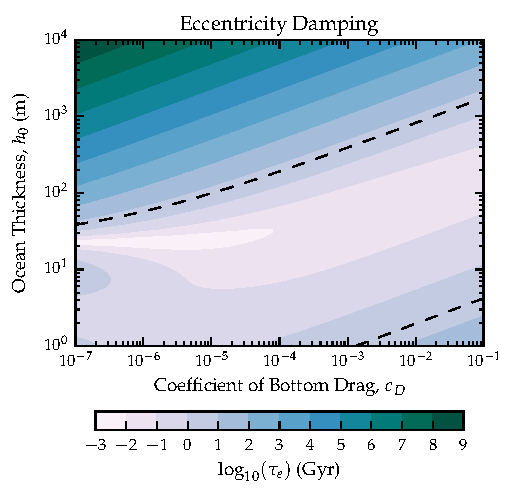
\includegraphics[width=0.55\linewidth]{Figures/eccentricity}
\caption{Characteristic eccentricity damping timescale for Titan, based on eccentricity tide ocean dissipation. The dashed contour represents the age of the Solar System, \SI{4.5}{\giga\year} \label{fig:edotTitan}}
\end{figure}

The characteristic eccentricity decay time scale, $\tau_e$, is shown in Figure \ref{fig:edotTitan}, where the dashed contour represents the age of the Solar System. Inward of the contour, decay times are less than \SI{4.5}{\giga\year}, with the $h_0 \sim \SI{22}{\metre}$ resonance having the shortest decay time of as little as \SI{1}{\mega\year}. Clearly this resonance would result in a much smaller eccentricity than we observe today. Outside of the region enclosed by the dashed contour, decay time scales exceed the maximum likely age of Titan, which can be no greater than the age of the Solar System. If we consider the thick ocean scenarios of $h_0 \gtrsim \SI{100}{\kilo\metre}$ from \citet{baland2014titan, sohl2014structural} then we would expect decay time scales on the order of \SI{e9}{\giga\year} or more based on Figure \ref{fig:edotTitan}, corresponding to virtually no change in eccentricity over the age of the Solar System. This is consistent with the high eccentricity observed today. Clearly, ocean dissipation has a negligible effect on Titan's eccentricity, and any change in $e$ likely comes from dissipation in the solid regions of the satellite, interaction with the other Saturnian satellites, or directly from dissipation in Saturn itself. 

To summarise the above discussion, if we assume the thick ocean scenario from \citet{sohl2014structural} and \citet{baland2014titan}, then Figure \ref{fig:a_evo} indicates that eccentricity and obliquity tide induced gravity-wave resonances will not significantly reduce the rate of semimajor axis change for Titan. For optimal bottom drag coefficients of $c_D = $ \numrange{e-2}{e-4}, however, the Rossby-wave resonance is capable of reducing the Saturn induced outward migration rate by up to \SI{40}{\percent}, regardless of the ocean thickness. Measurement of $da/dt$ would allow us to constrain the bottom drag coefficient for Titan's ocean because this Rossby-wave resonance becomes independent of ocean thickness, although no accurate measurement yet exists. For thick oceans, eccentricity damping from ocean dissipation is virtually non-existent, which is consistent with Titan's present day eccentricity.